% $Id$
%=============================================================================
\section{Software component definition}
%=============================================================================

Software components are the main part in CBSE. Therefore, we need a precise 
definition of this term.
Unfortunately, there are several different component definitions in 
literature.
A major problem is the multiple overloading of the term {\it Component} in the 
software world.


%------------------------------------------------------------------------------
\subsection{Syntactic specification of software components}
%------------------------------------------------------------------------------

Clemens Szyperski \cite{Szyperski02} defines a component by enumerating the 
characteristic properties of a software component:
\begin{description} 
\item [Definition (Szyperski)] A software component is a unit of composition 
with contractually specified interfaces and explicit context dependencies only.
A software component can be deployed independently and is subject to composition
by third party.
\end{description}

\begin{figure}[htbp]
    \begin{center}
        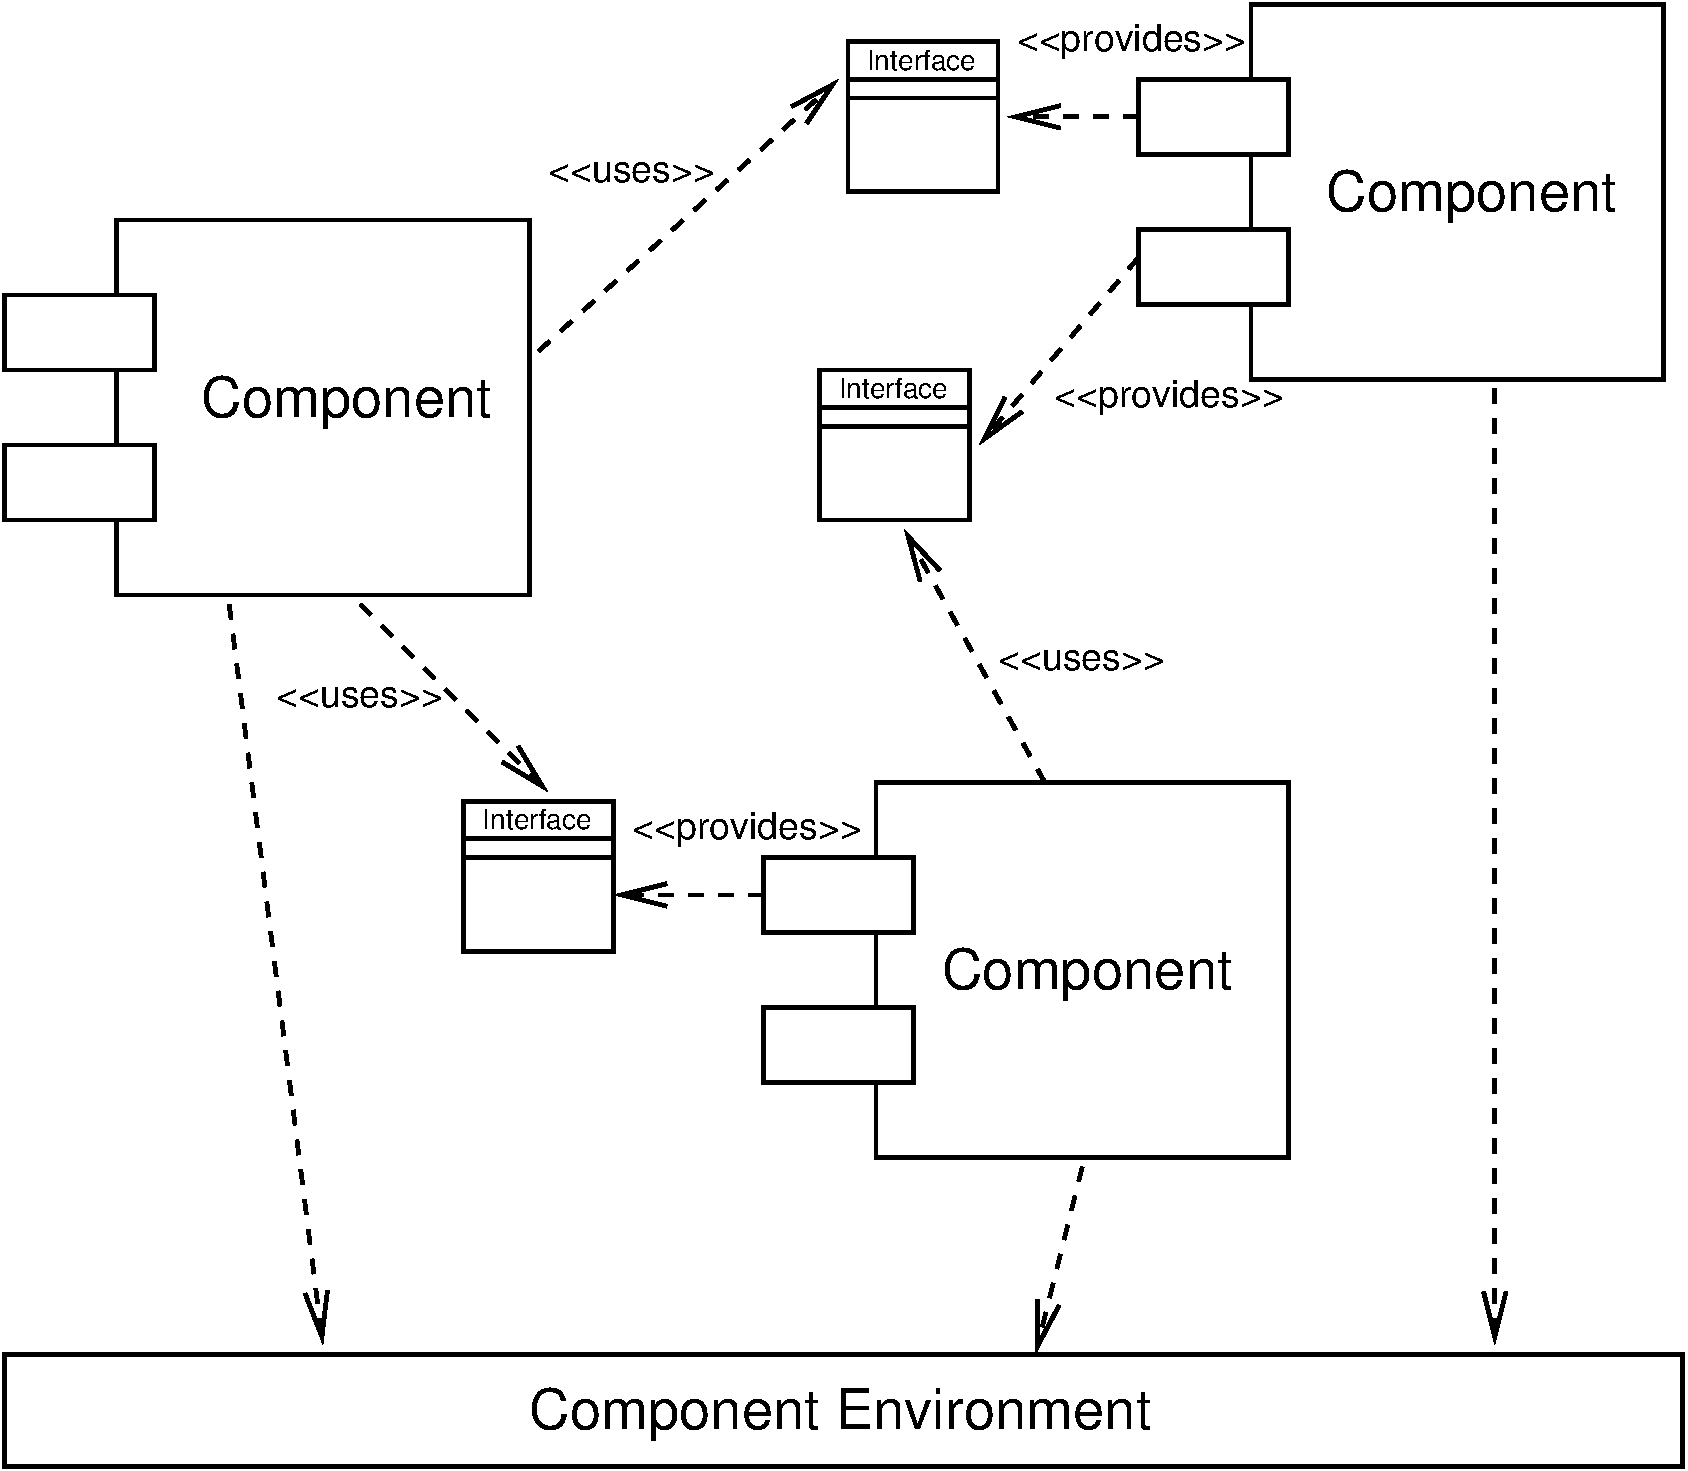
\includegraphics [width=7cm,angle=0] {figures/Environment}
        \caption{ A software component is a unit of composition 
	with contractually specified interfaces and explicit context 
	dependencies only.}
        \label{ComponentDef}
    \end{center}
\end{figure}

\noindent
This component definition contains important terms which must be discussed 
in detail \cite{ServerComponentPatterns02}:
\begin{itemize}
\item {\bf A unit of composition}:
The purpose of components is to be composed with other components.
A component--based application is thus assembled from a set of
collaborating components.

\item {\bf Contractually specified interfaces:}
To be able to compose components into applications, each component must provide
one or more interfaces.
These interfaces form a contract between the component and its environment.
The interface clearly defines which services the component provides - 
it defines its responsibilities.

\item {\bf Explicite context dependencies only:}
Software usually depends on a specific context, such as the availability of
database connections or other system resources.
One particularly interesting context is the set of other components that
must be available for a specific component to collaborate with.
To support the composability of components, such dependencies must be
explicitly specified.

\item {\bf Can be deployed independently:}
A component is self--contained. Changes to the implementation of a component
do not require changes to other components, as long as the interface remains
compatible.

\item {\bf Third parties:}
The engineers who assemble applications from components are not necessarily 
the same as those who created the components.
Components are intended to be reused - the goal is a kind of component
marketplace in which people buy components and use them to compose their own 
applications.

\end{itemize}



Szyperski's definition does not have satisfactory support for specification of
nonfunctional properties. 
The following definition, introduced by Ivica Crnkovic \cite{IVICA2002}, 
summarize the common aspects of component definitions, including 
nonfunctional features, found in literature:
\begin{description} 
\item [Definition (Crnkovic)]: 
To be able to describe a component completely and to ensure its correct
integration, maintenance and updating, the component should consist of
the following elements:
	\begin{itemize}
	\item A set of interfaces provided to, or required from, 
	the environment.
	These interfaces are particularly for interaction with other components,
	rather than with a component infrastructure or traditional software
	entities.
	\item An executable code, which can be coupled to the code of other 
	components via interfaces.
	\end{itemize}
	To improve the component quality, the following elements can be included
	in the specification of a component:
	\begin{itemize}
	\item The specification of nonfunctional characteristics, which are 
	provided and required.	
	\item The validation code, which confirms a proposed connection to 
	another component.
	\item Additional information, which includes documents related to the 
	fulfilling of specification requirements, design information, and use 
	cases.
	\end{itemize}
\end{description}

\noindent
A difficulty in CBSE is deciding how to deal with nonfunctional aspects
of communication, cooperation, and coordination included in a component
architecture.
These nonfunctional properties should be possible to compose and easy to
control.
A clear separation of nonfunctional requirements gives a component more
context independence.


%------------------------------------------------------------------------------
\subsubsection{Semantic specification of software components}
%------------------------------------------------------------------------------

Most techniques for describing interfaces are only concerned with the
signature part, in which the operations provided by a component's interface
are described, and thus fail to address the overall behavior of the component.
Ivica Crnkovic describes five levels of formalism for such 
semantic specification:
\begin{itemize}
\item {\bf No semantics}: The focus is exclusively on the syntactic parts of the
interfaces, represented by interface description or programming languages.
\item {\bf Intuitive semantics}: Here we use plain text, unstructured 
descriptions and comments about a component and its parts.
\item {\bf Structured semantics}: The semantics are presented in a structured 
way but need not be in accordance with any particular syntax or formalism.
\item {\bf Executable semantics}: The semantic aspects are expressed in a way 
that can be executed and verified by the system during run time (assertions 
can be used to express preconditions and postconditions and to test them during 
run time). Note that client code may also take advantage of executable 
assertions by checking the pre- and postconditions of an operation call.
\item {\bf Formal semantics}: Programs can be proved to have consistent and 
sound semantics. Formal specification languages such as VDM and Z are examples 
of approaches on this level \cite{ZNotation}.
\end{itemize}

\noindent
Specifications that include syntactic and semantic information are often called 
{\bf Contracts}.
As mentioned by Meyer \cite{OOSC97}, a contract lists the global constraints
that the component will maintain (the invariant).
For each operation within the component, a contract also lists the constraints
that need to be met by the client (the precondition) and those the component
promises to establish in return (the postcondition).



%------------------------------------------------------------------------------
\subsubsection{Objects versus components}
%------------------------------------------------------------------------------
The term {\it Object} and {\it Component} are often thought to be very similar,
but there are significant differences:
\begin{itemize}
\item {\bf Granularity.}
In contrast to a programming language object, a component has a much larger 
granularity and therefore usually more responsibilities.
Components were introduced to group objects to larger entities to reduce the
overall complexity of a software system. 

\item {\bf Multiple interfaces per component.}
An object typically implements a single class interface, which may be related
to other classes by inheritance.
In contrast, a component can implement many interfaces, which need not be 
related by inheritance.
Components can provide navigation operations to move between different 
component interfaces.
Navigation in objects is limited to moving up or down an inheritance tree
via cast or narrow operations.

\item {\bf Extensibility.}
While objects are implemented in a particular programming language,
components are not restricted in that way.
Components can be viewed as providers of functionality that can be 
replaced with equivalent components written in any programming language.
This extensibility is facilitated via the {\bf Extension Interface} design
pattern \cite{POSA2}, which defines a standard protocol for creating,
composing, and evolving groups of interacting components.

\item {\bf Improved communication.}
Components have a more extensive set of intercommunication mechanisms 
(synchronous/asynchronous, local/remote, messages/methods) 
than objects. 

\item {\bf Higher--level execution environment.}
Component models define a runtime execution environment, called component 
container, that operates at a higher level of abstraction than access via
ordinary objects.
The container provides additional levels of control for defining and
enforcing policies on components at runtime. 
\end{itemize}



%------------------------------------------------------------------------------
\subsubsection{A taxonomy of components}
%------------------------------------------------------------------------------

Because of its generic definition, the term component is used to describe
rather different software concepts.
The component taxonomy shown in Fig.~\ref{ComponentTaxonomy} should 
help to structure the diffent concepts in context of software components.

\begin{figure}[htbp]
    \begin{center}
        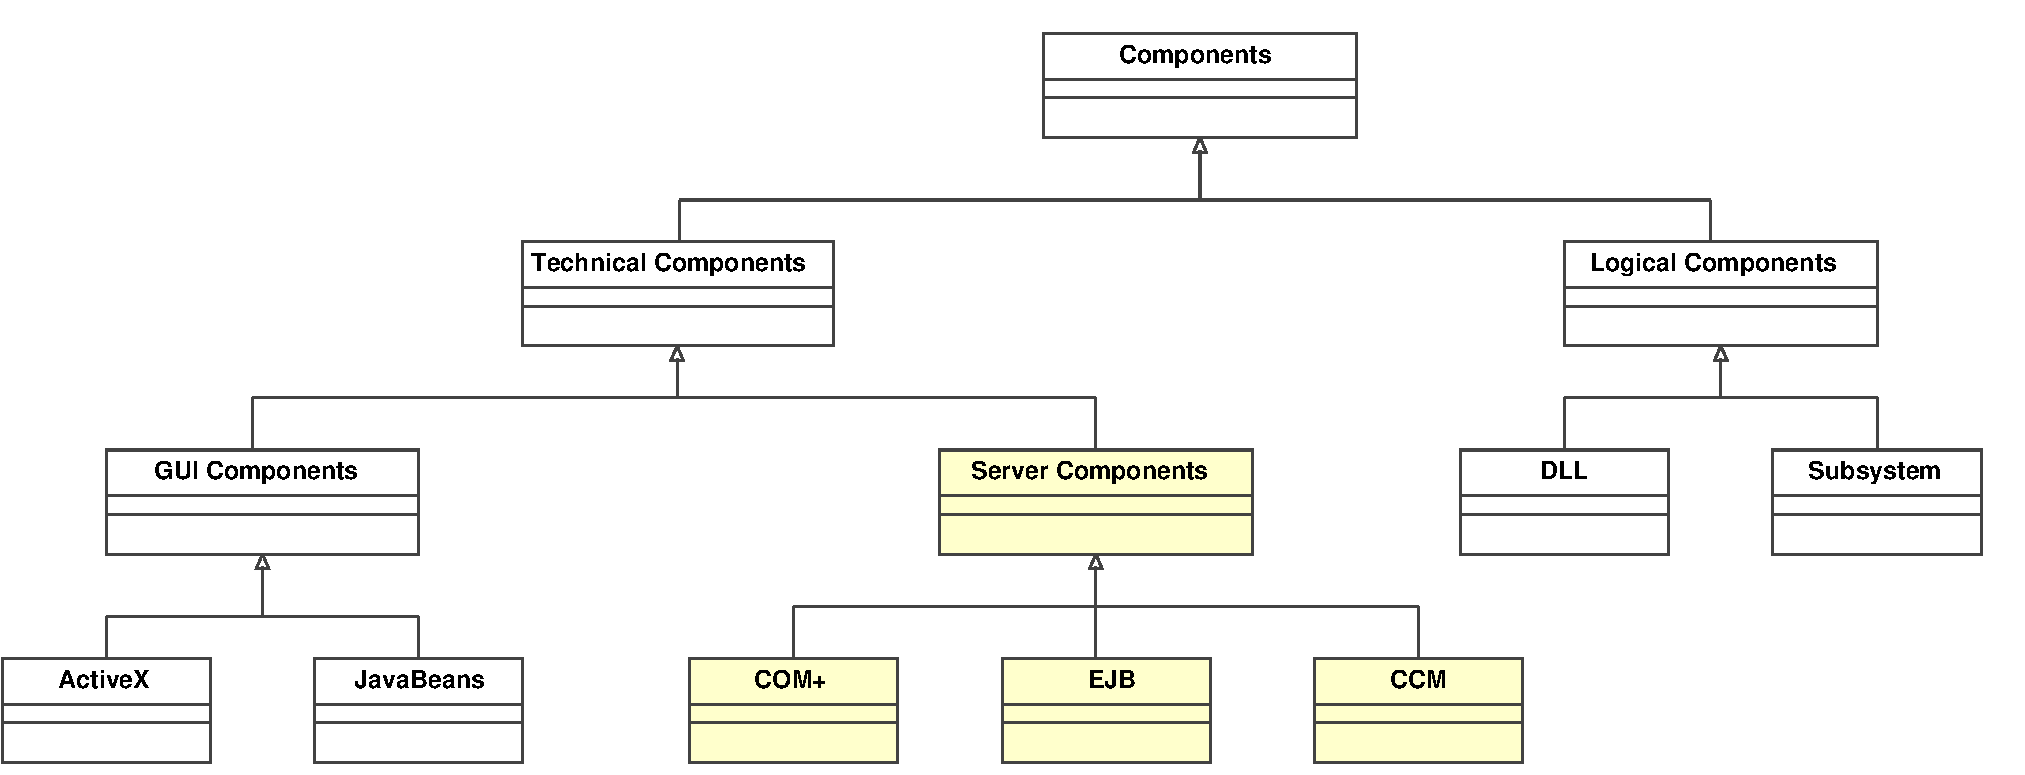
\includegraphics [width=15cm,angle=0] {ComponentBasedSoftwareEngineering/uml/ComponentTaxonomy}
        \caption{A taxonomy of components.}
        \label{ComponentTaxonomy}
    \end{center}
\end{figure}

\begin{itemize}
\item {\bf Logical Components:}
A logical component is simply a package of related functionality.
In can be some kind of {\bf Subsystem}, a {\bf DLL} or a complete, 
standalone application that runs as part of a larger system.
Logical components are mainly a way to keep the complexity of a system under 
control, and to organize version control or project management issues.
There is also the notation of a {\bf Business Component} \cite{HerzumSims99} - 
an aggregation of data, domain and user components that embody a complete
subsystem.

\item {\bf Technical Components:}
These are technical building blocks to asembly applications.
A technical component can not run without a runtime environment called 
container. A container handles the technical concerns like transactions,
security, failover or load--balancing for the components.
Technical components are either used in client applications or on the server.
\begin{itemize}
  \item {\bf Client components:}
  the container for client components is typically an IDE where the 
  components are configured at development time.
  The most popular examples are {\bf ActiveX Controls} and {\bf JavaBeans}

  \item {\bf Server components:}
  usually encapsulate business logic in multi--tier 
  systems and the container is typically a part of an application server.
  There are three mainstream component technologies: {\bf COM+}, 
  {\bf Enterprise JavaBeans} (EJB) and {\bf CORBA Component Model} (CCM).
  These server components are never used as client components, because
  the containers are rather complex and not available at the client side.
\end{itemize}
\end{itemize}


